ex\section{The Intervention Problem}
\label{sec:problemstatement}
Following STRIPS \cite{fikes1971strips}, we define a planning problem as a tuple $ P = \langle F, A, I, G \rangle$ where $F$ is the set of fluents, $I\subseteq F$ is the initial state, $G  \subseteq F$ represents the set of goal states and $A$ is the set of actions. Each action $a \in A$ is a triple $a=\langle Pre(a), Add(a), Del(a)\rangle$ that consists of preconditions, add and delete effects respectively, where $Pre(a), Add(a), Del(a)$ are all subsets of $F$. An action $a$ is applicable in a state $s$ if preconditions of $a$ are true in $s$; $pre(a) \in s$. If an action $a$ is executed in state $s$, it results in a new state $s^{\prime} = (s \setminus del(a) \cup add(a))$.  The solution to $P$ is a plan $\pi = \{a_1, \dots ,a_k\}$ of length $k$ that modifies $I$ into $G$ by execution of actions $a_1, \dots ,a_k$.  

Ramirez and Geffner \shortcite{ramirez2010probabilistic} formally defined a planning based approach for \textbf{goal recognition}, which is a tuple $T= \langle D, \mathcal{G}, O, Pr \rangle$ where $D=\langle F, A, I \rangle$ is a planning domain, $\mathcal{G}$ is the possible set of goals, and $\mathcal{G} \subseteq F$. $Pr$ is a prior probability distribution over the set of goals $\mathcal{G}$. An observation sequence $O = o_1, \ldots , o_m$ are actions $o_i \in A, i \in[1,m]$. A solution to the goal recognition problem is a probability distribution over $G \in \mathcal{G}$ indicating the relative likelihood of the goals in $\mathcal{G}$.

We also use the definiton for landmarks by Hoffman et al. \shortcite{hoffman2004lm}, which are propositions that have to be true at some time in every solution plan in a planning problem. Formally: a fact $L_P \subset F$ of a planning task $ P = \langle F, A, I, G \rangle$ is a \textbf{fact landmark} for $P$ iff $L_P$ is true in some state in all valid plans that modifies $I$ to $G$. We will use this definition to define features that identify actions that warrant intervention (described later).

The plan intervention problem ($\mathcal{I}$) is an extension to the goal recognition problem, which specially focuses on \textit{timely recognition} (i.e., the time the observer recognizes  that the user will reach $G_u$). Since we are using intervention to alert the user we need to minimize false negatives (caused by alerting too late) and false positives (caused by alerting too early) during recognition. We first define the plan intervention problem $\mathcal{I}$ for a multi-agent domain, where two competing agents (user and attacker) operate and later present the spacial case, where the only actor in the domain is a user.

A \textbf{common prefix} ($\phi$) for plans $\pi_g$ and $\pi\prime_{g\prime}$ for planning problems $P_g$ and $P_{g\prime}$ respectively is a sequence of actions such that $\phi$ is a prefix of $\pi_g$ and $\pi\prime_{g\prime}$. Otherwise $\phi=\emptyset$.

In the multi-agent case, the domain has a user agent $A_d$ and an attacker agent $A_u$. The user solves the planning task $ P_d = \langle F_d, A_d, I_d, G_d \rangle$. The attacker solves the planning task $ P_u = \langle F_u, A_u, I_u, G_u \rangle$. Note that because $\langle F_d, A_d, I_d\rangle \neq \langle F_u, A_u, I_u\rangle$, there can be many relationships between solutions to $P_d$ and $P_u$ ($\pi_d$ and $\pi_u$ respectively). For instance, in our blocks-words domain example, the hidden block gives the attacker additional actions to be used against the user. In this work we assume that $\pi_d$ and $\pi_u$ shares a common prefix $\phi$. However, there are actions $a\in\pi_u$ and $a \notin \phi$, such that if executed will divert the user away from $G_d$ and toward $G_u$. In other words, the attacker can leverage the progress the user had made to further its own goal.


\textbf{Plan intervention problem} $\mathcal{I} = \langle D, O, G_u, G_d \rangle$ consists of a planning domain $D$ and a sequence of observed actions  $O$, a set of undesirable states $G_u \subseteq F$, a set of desirable states $G_d \subseteq F$ ($G_u \neq G_d$). A solution to $\mathcal{I}$ is a vector of decision points corresponding to actions in $O$ indicating whether each action was identified as requiring intervention. 

The intervention problem makes several assumptions about the three actors. (1) \textbf{Observer}: intervention decisions are made in an online setting when observations appear incrementally and include actions executed by the attacker or the user. The goals $G_d$ or $G_u$ are known. The domains are discrete and actions are unit cost. The observer has full observability. (2) \textbf{User}: Follows a precompiled plan to reach $G_d$, but may reach the hidden $G_u$ unwittingly. The user likes the observer's help to avoid $G_u$. The user does not have full observability of the domain (3) \textbf{Attacker}: Follows a plan to reach $G_u$, that has a common prefix with the user's plan for $G_d$. Both the user and the attacker stick to their own plans, which means during execution they do not change their own plans or goals. The user and the attacker can follow either optimal and suboptimal plans to reach their goals.

\section{Modelling the Intervention Decision Space}
\label{sec:stategraph}
We introduce two methods, Full and Partial Methods to predict intervention.
\subsubsection{Full Method}
To assess the criticality of the current state to cause $G_u$, the observer enumerates action sequences that will transform the current state to $G_d$. These action sequences and intermediate states make up the observer's decision space, which is a single-root directed acyclic connected graph $S= \langle V,E \rangle$, where $V$ is the set of vertices denoting possible states the user could be in until $G_d$ is reached, and $E$ is the set of edges representing actions from $A$. We refer to this graph as the \textit{intervention graph}. The root of the intervention graph indicates the current state. Leaves of the graph are goal states (i.e., $G_u$ and $G_d$). A path from root of the tree to $G_u$ represents a candidate attack plan, while a path from root to leaf node containing $G_d$ represents a desirable plan.

%Algorithm \ref{bsg} describes how the intervention graph is built. 
The intervention graph is constructed similar to the relaxed planning graph (RPG) \cite{bonet01planningas}, where each level consists of predicates that have been made true and actions $a\in A$ whose preconditions are satisfied. Initially, before any observations have been made, the current state (i.e., root of the tree) is set to initial state $I$. Next, using the domain theory $D$, actions  $a\in A$ whose preconditions are satisfied at current state are added to the graph, ignoring delete effects. Each action in level $i$ spawn possible states for level $i+1$. Calling the method recursively for each state until $G_d$ and $G_u$ are added to some subsequent level in the graph will generate a possible hypotheses space for the observer. As a new observation arrives, the root of the graph is changed to reflect the new state after the observation and subsequent layers are also modified to that effect.
%\begin{algorithm}[tb]
%\scriptsize
%	\caption{Build Intervention Graph}
%	\label{bsg}
%	\begin{algorithmic}[1]
%		\Require $D$, $s$, $G_u$, $G_d$
%		\State $i=0;$ $ s_{i} \gets I $
%		\Procedure{expandgraph}{$D,s,G_u,G_d$}
%		\If{$s_{i} \models G_u,G_d$} return $\langle V,E\rangle$
%		\Else
%			\For{$a \in A$ where $Pre(a) \in s_{i}$}
%				\State \parbox[t]{0.95\linewidth} 
%				{$s_{i+1} \gets ((s_{i} \setminus Del(a))\cup Add(a))$}
%				\If{$s_{i+1} \equiv s_{i}$} continue \EndIf
%				\State $v \gets$ AddVertex ($s_{i+1}$)
%				\State $e \gets$ AddEdge ($s, s_{i+1}, a$)
%				\State $V \cup \{v\}$ $; E \cup \{e\}$
%				\State ExpandGraph ($D, s_{i+1}, G_u, G_d$)
%			\EndFor
%		\EndIf	
%		\EndProcedure
%	\end{algorithmic}
%\end{algorithm}


\subsubsection{Partial Method}
The Full method suffers from state space explosion since the observer attempts to enumerate the full decision space in large domains (e.g., Rush Hour puzzle). To overcome this problem, we propose the partial method. Instead of sampling plans from the full plan space, the observer samples only a subset of plans to compute a new feature vector.

\section{Domain Independent Features - Full Method}
We extract a set of features from the intervention graph that help determine when to intervene. These features include: Risk, Desirability, Distance to $G_d$, Distance to $G_u$ and Percentage of active undesirable landmarks in current state. We use these features to train a classifier that learns to identify intervention points. Figure \ref{fig:feature} illustrates a fragment of the intervention graph after \texttt{PICK-UP A}, which we will use as a running example to discuss feature computation.

\begin{figure}[tb]
	\centering{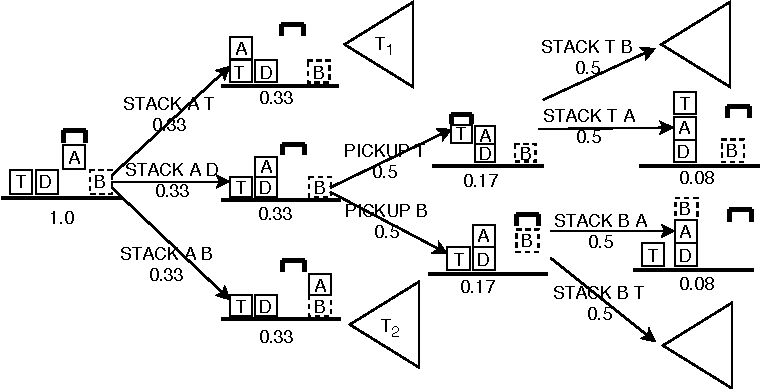
\includegraphics[width=\linewidth]{features.pdf}}
	\caption{Fragment of the decision space after PICKUP A has been observed for block-words example. Numbers under each state and action indicate the probability. Sub trees $T_1$ and $T_2$ are not expanded for simplicity.}
	\label{fig:feature}
\end{figure} 

\textbf{Risk ($R$)} quantifies how likely the effects of current observation will lead to $G_u$. $R$ is also coupled with the uncertainty the observer has about the next observation. We model the uncertainty as a uniform probability distribution across the set of actions whose preconditions are satisfied in current state. We define $R$ as the posterior probability of reaching $G_u$ while the user is trying to achieve $G_d$. Given the intervention graph, we extract paths from root to any leaf containing the $G_d$, including the ones in which the user has been subverted to reach $G_u$ instead. By virtue of construction termination, $G_d$ will always be a leaf.

Let $\Pi_{\mathcal{C}}$ be the candidate plans reaching $G_d$ and let $\left | \Pi_{\mathcal{C}} \right |=n$. The plan set $\Pi_{u}$ contains action sequences that reach state $G_u$ such that, $\Pi_{u} \subseteq \Pi_{\mathcal{C}}$, $\left | \Pi_{u} \right |=m$ and $(m<=n)$. We compute posterior probability of reaching $G_u$ for a path $\pi \in \Pi_{u}$, using chain rule in probability as, $P_{\pi}=\prod_{j=1}^{k}P(\alpha_j|\alpha_1, \alpha_2,...,\alpha_{k-1})$, and $\alpha_{j} \in A$ and $k$ is the length of path until $G_u$ is reached. Then: 
\begin{equation*} 
R = \left\{\begin{matrix} \frac{\sum_{i=1}^{m}P_{\pi_i}}{m} & m>0\\ 0 &  m=0 \end{matrix}\right.
\end{equation*}

According to example in Figure \ref{fig:feature}, $(n=6)$ and $(m=1)$. Since we assumed full observability for the observer, the root of the tree (current state) is assigned the probability of 1.0. Then, actions that are immediately possible after current state are each assigned probabilities following a uniform distribution across the branching factor (0.33). Then for each applicable action in the current state, the resulting state gets the probability of ($1.0\times0.33=0.33$). Similarly, we apply the chain rule of probability for each following state and action level in the graph until $G_u$ first appears in the path. $R=\frac{0.08}{1}=0.08$.


\textbf{Desirability ($D$)} measures the effect of the observed action to help the user pursue the desirable goal safely. Given $\Pi_{\mathcal{C}}$ as the set of plans extracted from the intervention graph that reach $G_d$ and $\left | \Pi_{\mathcal{C}} \right |=n$. The plan set $\Pi_{d}$ contains action sequences that reach state $G_d$ without reaching $G_u$, $\Pi_{d} = \Pi_{\mathcal{C}} \setminus \Pi_{u} $, we compute  posterior probability of reaching $G_d$ without reaching $G_u$ for a path $\pi \in \Pi_{d}$, using chain rule in probability as, $P_{\pi}=\prod_{j=1}^{k}P(\alpha_j|\alpha_1, \alpha_2,...,\alpha_{k-1})$, and $\alpha_{j} \in A$ and $k$ is the length of path. Then:

\begin{equation*} 
D = \left\{\begin{matrix}
\frac{\sum_{i=1}^{n-m}P_{\pi_i}}{n-m} & n-m>0\\ 
0 &  n-m=0
\end{matrix}\right.
\end{equation*} 

In Figure \ref{fig:feature}, there are five instances where user achieved $G_d$  without reaching $G_u$ (two in sub tree $T_1$, three in the expanded branch). Following the same approach to assign probabilities for states and actions, $D= \frac{(0.08+0.08+0.08+0.04+0.04)}{5} = 0.07$.

$R$ and $D$ are based on probabilities indicating the confidence the observer has about the next observation. We also use simple distance measures: (1) distance to $G_u$  ($\delta_u$) and (2) distance to $G_d$ ($\delta_d$). Both distances are measured in the number of actions required to reach a state containing $G_d$ or $G_u$ from root in the intervention graph.  

\textbf{Distance to $\boldsymbol{G_u}$} ($\delta_u$) measures the distance to state $G_u$ from the current state in terms of the number of actions. As with the computations of $R$ and $D$, given $\Pi_{\mathcal{C}}$ is the set of paths extracted from the intervention graph that reach $G_d$ and $\left | \Pi_{\mathcal{C}} \right |=n$. The path set $\Pi_{u}$ contains action sequences that reach state $G_u$ such that, $\Pi_{u} \subseteq \Pi_{\mathcal{C}}$, $\left | \Pi_{u} \right |=m$ and $(m<=n)$. We count  $s$, the number of the edges (actions) before $G_u$ is reached for each path $\pi \in \Pi_{u}$ and $\delta_u$ is defined as the average of the distance values given by the formula:
\begin{equation*} 
\delta_u = \left\{\begin{matrix}
\frac{\sum_{i=1}^{m}s_i}{m} & m>0\\ 
-1 &  m=0
\end{matrix}\right.
\end{equation*} 
In this formula, $-1$ indicates that the undesirable state is not reachable from the current state. For the example problem illustrated in Figure \ref{fig:feature}, $\delta_u=\frac{3}{1}=3$. 


\textbf{Distance to $\boldsymbol{G_d}$} ($\delta_d$) measures the distance to $G_d$ from current state. The path set $\Pi_{d}$ contains action sequences that reach $G_d$ without reaching $G_u$, $\Pi_{d} = \Pi_{\mathcal{C}} \setminus \Pi_{u} $, we count  $t$, the number of the edges where $G_d$ is achieved without reaching $G_u$ for each path $\pi \in \Pi_{d}$. Then, $\delta_d$ is defined as the average of the distances given by the formula:
\begin{equation*} 
\delta_d = \left\{\begin{matrix}
\frac{\sum_{i=1}^{n-m}t_i}{n-m} & n-m>0\\ 
-1 &  n-m=0
\end{matrix}\right.
\end{equation*}
In this formula, $-1$ indicates that $G_d$ can not be reached safely from the current state. For the example problem illustrated in Figure \ref{fig:feature}, $\delta_d=\left \lceil \frac{3+3+7+7+3}{5} \right \rceil=5$.


\textbf{Percentage of active attack landmarks} ($\mathcal{L}_{ac}$) captures the criticality of current state toward contributing to $G_u$. Landmarks \cite{hoffman2004lm} are predicates (or actions) that must be true in every valid plan for a planning problem. We used the algorithm in Hoffmann et al. \shortcite{hoffman2004lm} to extract fact landmarks for the planning problem $P = \langle D, G_u\rangle$. These landmarks are referred to as attack landmarks ($\mathcal{L}_{u}$) because they establish predicates that must be true to reach $G_u$.  Landmarks have been successfully used in deriving heuristics in plan recognition \cite{vered2018goalrec} and generating alternative plans \cite{bryce2014diverse}. We compute a feature using attack landmarks: percentage of active attack landmarks in current state ($\mathcal{L}_{ac}$). To compute $\mathcal{L}_{ac}$ for the example in Figure \ref{fig:feature}, we count the number of landmark predicates that have become active $(l)$ in the root of the intervention graph. Then, ($\mathcal{L}_{ac}$) is given by the formula: $\mathcal{L}_{ac} = \frac{l}{\left |\mathcal{L}_{u}\right|}$. In Figure \ref{fig:feature}, $l=4$ and $\mathcal{L}_{ac}=4/10=0.4$.

Algorithm~\ref{alg:exact} shows the computation of the exact feature vector for a given observation trace. The algorithm takes a PDDL domain, a set of undesirable and desirable states and a probability distribution as input and produces a relation $V$ of observations and feature vectors.

\section{Domain Independent Features - Partial Method} Risk and Desirability allow the observer to assess the likelihood the user will reach $G_d$ safely. For example, when there is no alternative path for the user to reach $G_d$ by avoiding $G_u$ from the current state, Risk value will be high. Howeve, these are intractible to compute in large problems. So we estimate them with plan distance measures. The intuition is that if the user is executing an unsafe plan (high risk), then the reference plan that is compatible with observations will be more similar to a sample of unsafe plans, compared to a sample of safe plans. We use action set distance, state sequence distance, causal link distance \cite{nguyen2012generating}, Generalized Edit Similarity for sequences of states and actions \cite{sohrabi2016finding} from the plan diversity literature as replacements for Risk and Desirability. We also use Landmark-Based Goal Completion Heuristic \cite{pereira2017} and number of actions to $G_u$ and $G_d$ as additional features.

The observer computes plan distances between a reference plan ($\pi^\prime$) and sampled plans ($\Pi^{\prime\prime}$) for both $G_u$ and $G_d$ for each incrementally revealed observation. We borrow from plan/goal recognition to produce $\pi^\prime$ and $\Pi^{\prime\prime}$ that agree with the observation history ($O$). Ramirez and Geffener \shortcite{ramirez2009plan} proposed an approach to compile the observations into the domain theory. Vered et al. \shortcite{vered2016mirror} proposed goal mirroring that concatenates a plan prefix, which agrees with the observations to a plan suffix, which is a plan generated from the last observed point in the prefix to the goal, that can be applied to both continuous and discrete domains. We follow the method proposed by Vered et al. \shortcite{vered2016mirror} in this work to generate observation compatible plans. We concatenate observation history with the optimal plan that reaches $G_u$ (and $G_d$) to produce $\pi^\prime$. Generating observation compatible $\pi^\prime$ and $\Pi^{\prime\prime}$ by compiling the observations into the domain theory is a possible extension to this work, which will be explored in the future. We use an off-the-shelf alternative planner to sample the plan space. Algorithm \ref{alg:apx} computes the partially estimated feature vector. For action, state sequence and causal link distances we use the median of all $<$reference, sample$>$ plan pairs as the feature value. We use the minim distance to goal state for all $<$reference, sample $>$ pairs. For action and state GED, we use the minim for all $<$reference, sample$>$ pairs.
\vspace{-2mm}
\begin{algorithm}[tb]
\scriptsize
	\caption{Build Full Vectors}
	\label{alg:exact}
	\begin{algorithmic}[1]
		\Require $D$, $I$, $O$, $G_u$, $G_d$, $p$-probability distribution.
		\Procedure{FeatureVector}{$D,O,I,G_u,G_d,p$}
		\State $i=0;$ $ s_i \gets I$
		\For{$o \in O$}
			\State $G(V,E) \gets ExpandGraph(D,s_i,G_u,G_d)$
			\State Apply action probabilities to $e\in E$ following $p$
			\State Apply state probabilities to $v\in V$ following $p$
			\State $\mathcal{V}(o) \gets \lbrack R_o,D_o,\delta_{u_o}, \delta_{d_o}, \mathcal{L}_{{ac}_o},Class\rbrack$
		\EndFor
		\EndProcedure
	\end{algorithmic}
\end{algorithm}
\setlength{\textfloatsep}{2pt}

\begin{algorithm}[tb]
\scriptsize
	\caption{Build Approximation Vector}
	\label{alg:apx}
	\begin{algorithmic}[1]
		\Require $D$, $s$, $G_u$, $G_d$
		\State $i=0;$ $ s_{i} \gets I $
		\State $prefix,suffix,\Pi^{\prime\prime}, \mathcal{V} \gets \varnothing$
		\Procedure{Partial}{$D,s,G_u,G_d,O$}
		\For{$o \in O$}
			\State \parbox[t]{0.95\linewidth}{$prefix \gets prefix + o$}
			\State \parbox[t]{0.95\linewidth} 
				{$s_{i+1} \gets ((s_{i} \setminus Del(o))\cup Add(o))$}
			\For {$ g \in \{G_u, G_d$\}}
				\State \parbox[t]{0.95\linewidth}{$suffix \gets OptimalPlan(s,g)$}
				\State \parbox[t]{0.95\linewidth}{$\Pi^\prime \gets prefix + suffix$}
				\State \parbox[t]{0.95\linewidth}{$\Pi^{\prime\prime} \gets \text{Observaton compatible alt. plans for } g$}
				\State \parbox[t]{0.95\linewidth}{$v_1 \gets$ MedianActionSetDist$(\Pi^\prime, \Pi^{\prime\prime})$}
				\State \parbox[t]{0.95\linewidth}{$v_2 \gets$ MedianCausalLinkDist$(\Pi^\prime, \Pi^{\prime\prime})$}
				\State \parbox[t]{0.95\linewidth}{$v_3 \gets$ MedianStateSequenceDist$(\Pi^\prime,\Pi^{\prime\prime})$}
				\State \parbox[t]{0.95\linewidth}{$v_4 \gets$ MinimumDistToState $(g,\Pi^{\prime\prime})$}
				\State \parbox[t]{0.95\linewidth}{$v_5 \gets$ MinimumActionGED $(\Pi^\prime, \Pi^{\prime\prime})$}
				\State \parbox[t]{0.95\linewidth}{$v_6 \gets$ MinimumStateGED $(\Pi^\prime, \Pi^{\prime\prime})$}
				\State $\mathcal{V}(o) \gets \lbrack v_1,v_2,v_3,v_4,v_5,v_6\rbrack $
			\EndFor
			\State \parbox[t]{0.95\linewidth}{$v_7 \gets$ AchievedLandmarkHeuristic $(G_u,s_{i})$}
			\State $\mathcal{V}(o) \gets \mathcal{V}(o)+\{v_7\}$
		\EndFor
		\EndProcedure
	\end{algorithmic}
\end{algorithm}